\documentclass{bioinfo}
\copyrightyear{2014}
\pubyear{2014}
\usepackage{amssymb}
\usepackage{algorithm}
\usepackage{algpseudocode}

\begin{document}
\firstpage{1}

\title[Sequence clustering by all pairs-search]{Starcode: sequence
clustering based on all-pairs search }
\author[Valera Zorita \textit{et~al}.]{Eduard Valera Zorita\,$^{1,2}$, Pol
Cusc\'o\,$^{1,2}$ and Guillaume Filion\,$^{1,2}$\footnote{to whom
correspondence should be addressed}}
\address{$^{1}$Genome Architecture, Gene Regulation, Stem Cells and
Cancer Programme, Centre for Genomic Regulation (CRG), Dr. Aiguader 88,
08003 Barcelona, Spain.\\
$^{2}$Universitat Pompeu Fabra (UPF), Barcelona, Spain.}

\history{Received on XXXXX; revised on XXXXX; accepted on XXXXX}

\editor{Associate Editor: XXXXXXX}

\maketitle

\begin{abstract}
\section{Motivation:}
The increasing throughput of sequencing technologies offers new
applications and challenges for computational biology. In many
of those applications, sequencing errors need to be corrected.
This is particularly important when using random DNA barcodes to
trace and quantify transcripts or lineages, since spurious barcodes
introduce inexistent entities. The reference population of random
barcodes is unknown and in this case, error correction amounts
to performing a pairwise comparison of all the barcodes,
which is unfeasible for excessive computationally complexity.

\section{Results:}
Here we address this problem and describe an exact algorithm to
determine which pairs of sequences lie within a given Levenshtein
distance. For error correction or redundancy reduction purposes,
matched pairs are then merged into clusters represented by a
canonical sequence. The effiency of starcode is attributable to
the poucet search, a novel implementation of the Needleman-Wunsch
algorithm performed on the nodes of a trie. On the task of matching
random barcodes, starcode outperforms sequence clustering algorithms
in both speed and precision.

\section{Availability and implementation:}
The C source code is available at http://github.com/gui11aume/starcode.

\section{Contact:} \href{guillaume.filion@gmail.com}{guillaume.filion@gmail.com}
\end{abstract}


\section{Introduction}

Sequencing technologies never achieve perfect precision. For instance,
the Illumina platform \citep{pmid16056220} has a 1-2\% error rate
consisting of substitutions \citep{pmid18660515, pmid21576222}
and the PacBio platform has a 15\% error rate consisting of insertions
and deletions \citep{pmid19023044}. The throughput of such technologies
has recently created additional needs to develop efficient error
correction algorithms.

Sequencing errors can be discovered by comparing the reads to a
reference genome. However, such a reference is not always available.
When the sequences are random or taken from an unknown source,
clustering is the main strategy to correct the errors.
For instance, this situation arises when using random barcodes to
track cells or transcripts \citep{pmid18809713, pmid23953119}.
Sequencing errors will create erroneous (nonexistent) barcodes
that have to be removed.

Sequence clustering can be viewed as a community detection problem
on graphs, where nodes represent sequences and edges represent matches
between related sequences. The process consists of a matching phase
(the most computationally intensive), where the graph is constructed,
and a clustering phase where communities are identified.

Here we describe a sequence clustering algorithm focused on error
correction. The algorithm is called ``starcode'' in reference to 
clusters of random barcodes, which typically have a star shape.
Starcode is based on all-pairs search, \textit{i.e.} all the pairs
of sequences below a given Levenshtein distance are identified during
the graph construction phase. Matching is carried out by lossless
filtration, followed by a trie search.  The novelty of the algorithm
is the poucet strategy, which uses the redundancy of alphabetically
sorted sequences to avoid unnecessary recomputations and gain speed.

In this article we present and benchmark starcode. We show that on
real biological datasets, starcode is faster than existing sequence
clustering software. Even though starcode was designed for error
correction, we show that it can be used for other problems. As an
illustration, we use it to identify enriched motifs in a bacterial
genome and in protein-RNA interaction experiments.

\begin{methods}
\section{Methods}
\subsection{Inexact string matching using tries}
The matching method of starcode is based on a variation of the
Needleman-Wunsch (NW) algorithm \citep{pmid5420325}. In the
original algorithm (Figure \ref{fig:NW}a), the Levenshtein
distance between two sequences is found by applying a recurrence
relation throughout a matrix of $mn$ terms (the edit matrix),
where $m$ and $n$ are the respective sequence lengths. The complexity
of this dynamic programming approach is $O(mn)$. 

\begin{figure}[!tpb]
\centerline{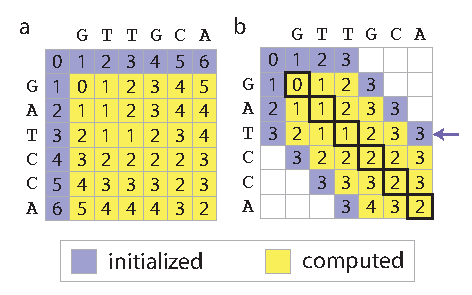
\includegraphics{NW.pdf}}
\caption{Needleman-Wunsch (NW) sequence comparison. \textbf{a}
Comparison of GTTGCA and GATCCA. The margins of the edit matrix
(purple) are initialized and the cells (yellow)
are computed from left to right and from top to bottom by the NW
dynamic programming algorithm. $E[i,j]$, the term of
coordinates $(i,j)$ is computed as
$\min(E[i-1,j]+1, E[i,j-1]+1, E[i-1,j-1]+\Delta(i,j))$, where
$\Delta(i,j) = 0$ if the $i$-th symbol from the first sequence is the
same as the $j$-th symbol from the second, and $\Delta(i,j) = 1$
otherwise. The Levenshtein distance between the two sequences is the
value of the bottom right cell. \textbf{b} Lower complexity algorithm
to determine whether GTTGCA and GATCCA are 2-matches.
The values in the purple cells are set
during initialization. The dynamic programming algorithm proceeds as
above, with the difference that it is aborted if the value of a
diagonal cell (bold borders) is larger than 2. The values in the
purple cells may differ from the original NW scheme (purple arrow),
but the values in the yellow cells are nevertheless identical.
The values of the white cells are never computed, which contributes to
reducing the complexity.}\label{fig:NW}
\end{figure}

In many instances, the information of interest is to find out
whether the sequences are $\tau$-matches (\textit{i.e.} their distance
is less then or equal to a fixed threshold $\tau$).
In that case, the complexity can be reduced to $O(\tau \min(m,n))$.
Instead of computing all the terms of the edit matrix, it is initialized
as shown on Figure \ref{fig:NW}b and only the terms around the diagonal
are computed. If a diagonal term has a value greater than $\tau$,
the process is halted because the sequences are not $\tau$-matches.

This method can be used to match sequences against a prefix tree,
also known as a trie \citep{ukkonen}. The terms of the edit matrix
are updated row-wise while a depth-first search traverses the trie
(Figure \ref{fig:trie}). Every time a node is visited,
a row is computed, and every time the search backtracks, a row is
erased. If the threshold value $\tau$
is exceeded for a diagonal term, the Levenshtein distance for all the
downstream sequences is also necessarily greater than $\tau$. Therefore,
no more hits are to be discovered in this path and the depth-first
search backtracks to the parent node. When the process halts, every
tail node (corresponding to a sequence of the database) on the path
of this search is a $\tau$-match of the query. This method is
efficient because it eliminates large areas of the search space, and
because the NW comparison of the query with each prefix of the database
is computed only once.

\begin{figure}[!tpb]
\centerline{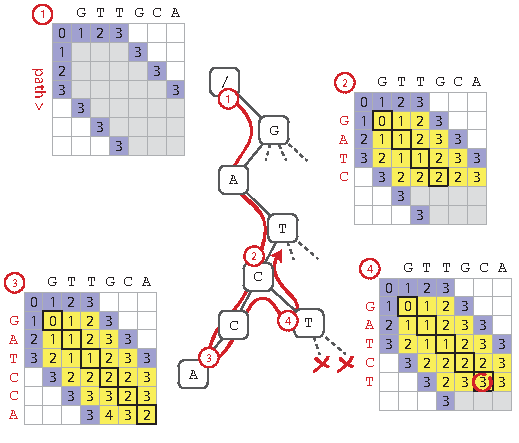
\includegraphics{trie.pdf}}
\caption{NW algorithm on tries. Each sequence of the index is a
path in the trie. The query GTTGCA is written at the top of the matrix,
which is initialized as shown on Figure \ref{fig:NW}b. The trie is
traversed by a depth-first search (red path). At each
depth, the node added to the path is written on the left of the edit
matrix and the row is computed. Checkpoints from 1 to 4 (circled red
numbers) show the state of the edit matrix as the search proceeds. The
node labeled 3 is a leaf and thus corresponds to a 2-match of the
query. After discovering the hit, the search path backtracks to the
node labeled 2 and the last rows of the edit matrix are erased.
The search path then goes to the node labeled 4, in which case the
newly computed diagonal cell exceeds the threshold (circled in red).
Even if this node has children, they are not visited (red crosses)
because there is no 2-match to discover.}
\label{fig:trie}
\end{figure}


\subsection{The poucet search algorithm}
The search strategy can be further improved. If two consecutive
queries share a prefix of length $k$, the succession of computations
up to the $k$-th row of the edit matrix will be exactly the same
for both queries. Therefore, computation intermediates can be
stored in the nodes of the trie, so that the next trie search can start
at depth $k$. However, storing the rows of the edit matrix in the nodes
meets some difficulty. Indeed, on the $k$-th row, the terms on the
right side of the diagonal depend on characters that are not shared
between the two queries. This issue is solved by storing in each
node a combination of row and column terms that form an angle shape,
looking like a horizontally flipped L (Figure \ref{fig:poucet}).
Using this structure, the computation intermediates stored in a
node at depth $k$ depend only on the first $k$ characters of the
query.

To take full advantage of this property, the input sequences are
sorted alphabetically, which maximize prefix sharing between
consecutive queries. In the fairy tale ``Le Petit Poucet'', the
hero seeds white pebbles for his older brothers to find their way
home, which is reminiscent of the way a smaller query (in alphabetical
order) paves the way for the next. We therefore called this search
algorithm ``poucet''.

\begin{figure}[!tpb]
\centerline{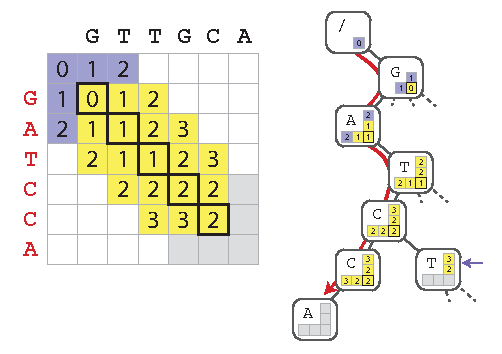
\includegraphics{poucet.pdf}}
\caption{Poucet search algorithm. The algorithm proceeds with the
same principles as shown on Figure \ref{fig:trie} with the difference
that the edit matrix is not updated row-wise, but along a horizontally
flipped L. As the depth-first search proceeds, these values
are stored in the nodes of the trie. Since the values in the vertical
part of the flipped L are the same for every child of a node,
they are computed only once (purple arrow). The values in the grey
cells will be computed as the search path (red) visits the node.
Storing the intermediates in the nodes allows the next query to
restart at depth $k$ if it shares a common prefix of length
$k$ with the current query.}
\label{fig:poucet}
\end{figure}


\subsection{Lossless filtration}
When a query has no match, it is advantageous to omit the trie
search. To this end, starcode uses a partition
approach similar to that described by \cite{WuManber1992}. If the
query is partitioned in $\tau+1$ segments, every $\tau$-match
contains at least one of those (assuming that all the segments
have length at least $\tau$). Indeed, there are at most $\tau$
differences between the query and the match, so at least one segment
is unmodified. In the $\tau$-match, the position of the shared
segment is at most $\tau$ nucleotides on the left or on the right
of its position in the query.

These observations are the basis of a filtration method that proceeds
as follows. Every time a sequence is added to the trie, its segments
are added to $\tau+1$ different indexes. More specifically, the
first $\tau$ nucleotides of the sequence are removed, and the rest
of the sequence is partitioned in $\tau+1$ segments of sizes
differing by at most 1 (the longer segments always in 3' for
consistency). The first fragments are added to the first index,
the second fragments to the second index \textit{etc}.

Before the search, segments of the query are looked up in
the indexes, and in case no match is found, the trie search is
omitted because this query has no $\tau$-match. If at least one
segment is found, the trie search is performed. As mentioned above,
segments shared between the query and a $\tau$-match can be shifted
up to $\tau$ nucleotides. For this reason, shifted segments are
looked up in the indexes according to the following scheme ensuring
that no match can be missed.
(Figure \ref{fig:filtration}). The rightmost segment is looked up
in the $\tau$+1-th index, the second rightmost segment and the
contiguous segments shifted by 1 nucleotides are are looked up in the
$\tau$-th index and so on until the first segment and its
contiguous segments shifted by up to $\tau$ nucleotides are
looked up in the first index.

\begin{figure}[!tpb]
\centerline{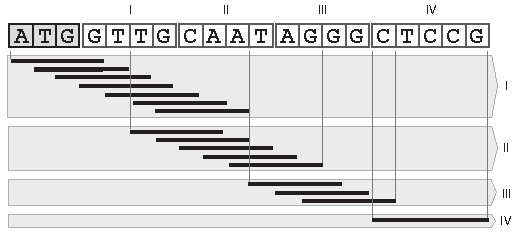
\includegraphics{filtration.pdf}}
\caption{Lossless filtration illustrated by an example sequence
of length 20 with $\tau=3$. The last $\tau$ nucleotides of the query
are removed, and the rest is divided into 4 series of contiguous
segments.  Each series is queried against a different index numbered
I to IV.  For instance, the only segment queried against index I
is GTTG, while those queried against index II are GCAA, CAAT and AATA.
If any of the segments is found in the appropriate index, the trie
search is performed, otherwise it is omited as there can be no
$\tau$-match. Regardless of the result, segments labelled I to IV
are then added to the corresponding respective index (\textit{i.e.}
only one segment is added to each index).}
\label{fig:filtration}
\end{figure}

\subsection{Seek and construct}
To reduce the size of the search space, starcode uses a dynamic
``seek and construct'' approach whereby queries are processed
meanwhile the trie is built. In other words, each sequence is
matched against the trie before it is inserted. If A and B are
mutual $\tau$-matches, either A will be queried when B is in
in the trie, or the converse. Either way, the match A-B is
discovered. This guarantees that every $\tau$-match is discovered,
while maintaining the trie as ``thin'' as possible, thereby reducing
the search time.  The whole matching process is summarized in
the pseudocode shown in Algorithms~\ref{alg:starcode} and
\ref{alg:poucet}.

\begin{algorithm}
  \caption{Starcode algorithm}
  \label{alg:starcode}
  \begin{algorithmic}[1]
    \State \textbf{Define:} $\tau$
    \State \textbf{Variables:} $seed$, $start = 0$,
    $height$, $seq$, $trie$, $lastseq$, $k$
    \State \textbf{Containers:} $hits$, $pebbles$
    \State \textsc{read} sequence file
    \State $height \gets$ \textsc{determine} maximum sequence length
    \State \textsc{pad} sequences up to $height$
    \State \textsc{sort} sequences alphabetically
    \State $k \gets$ \textsc{compute} lookup word lengths
    \State $trie \gets$ \textsc{create} an empty trie of height $height$
    \State \textsc{insert} root node of $trie$ in $pebbles$ at depth 0
    \ForAll{sequences}
    \State $seq \gets$ \textsc{get} next sequence
    \If{at least one $k$-mer of $seq$ is in the lookup table}
    \State $seed \gets$ \textsc{length} of shared prefix
    between current and next sequence
    \State $start \gets$ \textsc{length} of shared prefix
    between $seq$ and $lastseq$
    \State \textsc{clear} hits
    \State \textsc{clear} $pebbles$ at depth $>start$
    \ForAll{$pebbles$ at depth $start$}
    \State $node \gets$ \textsc{get} next node from $pebbles$
    \State \textbf{call} \textsc{poucet}($seq$, $node$, $seed$,
    $hits$, $pebbles$)
    \EndFor
    \State \textsc{process} $hits$ and \textsc{link} matches to $seq$
    \State $lastseq \gets seq$
    \EndIf
    \State \textsc{insert} $seq$ path in $trie$
    \State \textsc{insert} $seq$ $k$-mers into the lookup table
    \EndFor
  \end{algorithmic}
\end{algorithm}

\begin{algorithm}
  \caption{Poucet search algorithm}
  \label{alg:poucet}
  \begin{algorithmic}[1]
    \Procedure{poucet}{$query$, $node$, $seed$, $hits$, $pebbles$}:
    \State \textsc{compute} $node$-specific column following NW
        \Comment{Fig.1}
    \ForAll{$child$ nodes in $node$}
    \State \textsc{compute} $child$-specific row following NW
        \Comment{Fig.1}
    \State \textsc{compute} center value using row and column
        \Comment{Fig.1}
    \If{center value $>\tau$} \Comment{Mismatches exceeded.}
    \State \textbf{continue} with next $child$
    \EndIf
    \If{$node$ depth = $height$} \Comment{Hit found.}
    \State \textsc{save} $node$ sequence in $hits$
    \State \textbf{continue} with next $child$
    \EndIf
    \If{$node$ depth $\leq seed$}
    \State \textsc{save} $node$ in $pebbles$ at current depth
    \EndIf
    \State \textbf{call} poucet($query$, $child$, $seed$, $hits$, $pebbles$)
    \EndFor
    \EndProcedure
  \end{algorithmic}
\end{algorithm}


\subsection{Parallelization}
Queries are sorted and partitioned in contiguous blocks.
The matching step then proceeds in two phases. In the first, a
distinct trie is built from the sequences of each block according
to the algorithm described above. In the second, all the sequence
blocks are queried against the tries. If the queries are partitioned
in $N$ blocks, the first phase consists of $N$ seek and construct
jobs, wile the second consists of $N(N-1)/2$ query jobs. In each
phase, the jobs show little dependency on each other, so the
matching algorithm can be efficiently parallelized provided $N$
is larger than the number of independent threads.

\subsection{Clustering}
The default clustering algorithm of starcode is designed to correct
sequencing error. This method uses message passing \citep{mackay}
to identfy and count ``canonical'' sequences (also referred to as
centroids in the clustering terminology). Each sequence transfers its
read count to its closest $\tau$-match provided the latter has at least 5
times more counts. If the condition is not met, the transfer does
not take place. If the sequence has several equally close
$\tau$-matches, the counts are split equally among them. The
process is repeated recursively, starting from sequences with
lowest read count. The sequences with a positive read count at
the end of the process are considered canonical. Clusters consist
of all the sequences transferring their read counts to the same
canonical sequence (sequence transferring their read counts to
different canonicals are discarded). Note that the radius of the
clusters can be higher than the maximum distance used for matching.

Since no sequencing technology has an error rate higher than 20\%,
it is expected that sequences appearing from sequencing errors will
always have 5 times or lower read count than the canonical sequence.
Otherwise, sequences are more likely unrelated, or both derived from
the same canonical sequence. 

For other sequence clustering problems, starcode implements a
multi-purpose algorithm called ``sphere clustering''
\citep{pmid23953119}. In sphere clustering, sequences are sorted by
frequency of occurrence. Starting from the most
frequent, each sequence becomes canonical and claims all its
$\tau$-matches, which forms a cluster of radius $\tau$ (hence the
name). Claimed sequences are immediately removed, so that they can
belong to only one cluster.


\end{methods}

\section{Results}

\subsection{Benchmark conditions}
All the tests were performed on a 16-core dual-processor
Intel Xeon E5-2687W v2 system with 256~GB of DDR3-RAM at
1866~Mhz. Command-line parameters were set equivalently in all
softwares to run in single-core mode allowing up to 3 mismatches for
input sequences of length 50. Execution options used in simulation and
real datasets are summarized in Table \ref{tab:params1} and Table
\ref{tab:params2}, respectively.

\begin{table}[h]
\centering
\caption{Software execution options used in simulation benchmark.}
%\resizebox{\columnwidth}{!}{
\begin{tabular}{l|l}
    \bf{software} & \bf{execution options}\\
    \hline
    starcode & \texttt{starcode -d3}\\
    slidesort & \texttt{slidesort\_v2 -d 3 -t E -c DNA}\\
    CD-HIT 4.6.1 & \texttt{cd-hit-est -n 9 -c 0.9 -M 0 -r 0}\\
    SEED & \texttt{SEED --mismatch 3}\\
\end{tabular}
%}
\label{tab:params1}
\end{table}

\begin{table}[h]
\centering
\caption{Software execution options used in real data benchmark.}
%\resizebox{\columnwidth}{!}{
\begin{tabular}{l|l}
    \bf{software} & \bf{execution options}\\
    \hline
    starcode & \texttt{starcode -d3}\\ 
    slidesort & \texttt{slidesort\_v2 -d 3 -u -t E -c DNA}\\
    CD-HIT 4.6.1 & \texttt{cd-hit-est -n 8 -c 0.94 -M 0}\\
    SEED & \texttt{SEED --mismatch 3 --shift 3}\\ 
\end{tabular}
%}
\label{tab:params2}
\end{table}

\subsection{Presentation and basic performance}
\label{performance}
Starcode is a general purpose DNA sequence clustering tool with a
strong focus on error correction. Errors are assumed to be mismatches,
insertions or deletions (the implementation presented here matches
sequences with up to 8 errors). The input sequences can be single
or paired-end reads, with an upper limit of 1024 nucleotides (512
for paired-end). Sequences may be of variable length, they may
be trimmed and filtered for quality or not. Input formats may be raw
sequence, fasta or fastq (in which case starcode ignores the quality).
By default, starcode outputs sequence clusters, it can also be used
to filter out redundant sequences from input files. By default,
clustering is performed under the assumption that divergence occurs
from experimental errors (sequencing errors, PCR mutations
\textit{etc}), a more general algorithm is also available for other
clustering problems (an example of which is given in section
\ref{section:motifs}).

We show the basic performance and scalability of starcode on a
dataset of pseudo random sequences (Figure \ref{fig:perf}). The standard
configuration is a set of 1,000,000 sequences of length 40, running
on 1 thread and with a maximum Levenshtein distance of 3. Only one
parameter is modified whereas the others were kept constant. 

Figure \ref{fig:perf}a shows the running time of starcode as a
function of the number of input sequences $n$. In double logarithmic
scale the trend is a straight line with slope 1.5, suggesting that the
running time complexity of starcode is lower than quadratic (the
naive implementation of all-pairs search). Note that the sequences of
this dataset have no match, see section \ref{section:benchmark} for
an evaluation of the performance on more realistic datasets.
Figure \ref{fig:perf}b shows that the running time grows exponentially
as a function of the maximum Levenshtein distance used for clustering.
The reason is that the trie fans out exponentially and the search bails
out at a greater depth as the maximum distance increases.
As a function of the sequence length, the running time first increases 
but then plummets and stays low (Figure \ref{fig:perf}c). Beyond a
threshold length, the filtering algorithm starts to be efficient, and
most of the queries are resolved without searching the trie.
Finally, we show the scalability of starcode with increasing number
of threads in Figure \ref{fig:perf}d. The search algorithm is fully
parallel and the relative performance increases linearly up to 12 threads.
The bending observed thereafter has two sources. The first is 
that the input reading and clustering steps are brief but not parallel,
the second is that there is insufficient memory bandwidth to satisfy
the increased demand of memory accesses due to hardware limitations.

\begin{figure}[!tpb]
% Basic performance figure.
\centerline{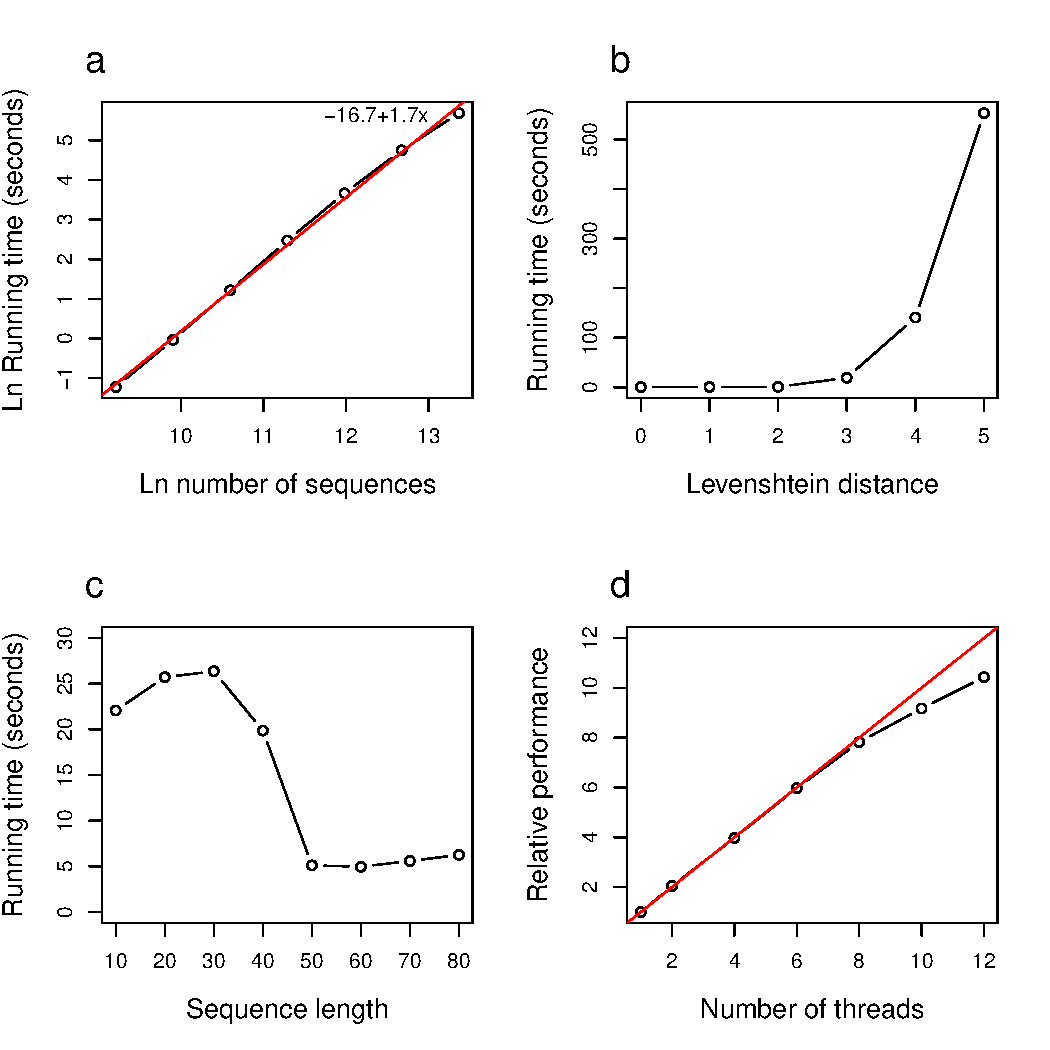
\includegraphics[scale=0.47]{scalability.pdf}}
\caption{Scalability. \textbf{a} Logarithm of the running time versus the
logarithm of the number of sequences to be clustered. \textbf{b}
Running time as a function of the clustering distance. \textbf{c}
Running time versus length of the input sequences. \textbf{d} Relative
performance increase for different number of parallel threads. 
}\label{fig:perf}
\end{figure}

\subsection{Benchmark}
\label{section:benchmark}
We benchmarked starcode against the sequence clustering algorithms
slidesort \citep{pmid21148542}, seed \citep{pmid21810899},
rainbow \citep{pmid22942077} and cd-hit \citep{pmid23060610}. Even though
slidesort is an all-pairs search algorithm, it was included in the
benchmark because sequence comparison is the most computationally
intensive step of the sequence clustering problem. Rainbow runs
exclusively on paired-end reads, while the other tools run on single
reads.

%% Synthetic data %%
The performance of sequence clustering algorithms can be sensitive
to the size of the clusters in the dataset, which in many applications
is not known \textit{a priori}. We therefore set up a benchmark on
artificial datasets to test the accuracy and the scaling of the
tools on a known cluster structure. We generated 4 datasets of 1 million
50-mers arranged in 1 to 1,000 clusters. Each cluster consisted
of 100 repeats of the same centroid sequence, plus satellites
derived from the centroid by incorporating 3 errors including at
most 1 indel. The number of satellites per cluster ranged from
999900 to 900. Evaluating the exactness of slidesort on these datasets
was problematic because the number of 3-matches in each dataset is
not known (pairs of statellites in the same cluster may be 3-matches
or not). For this reason we only compared the number of pairs found
by starcode with the number of pairs found by slidesort. The 
outcome of the test is summarized in
Figure \ref{fig:benchmark}.

\begin{figure}[!tpb]
  \centerline{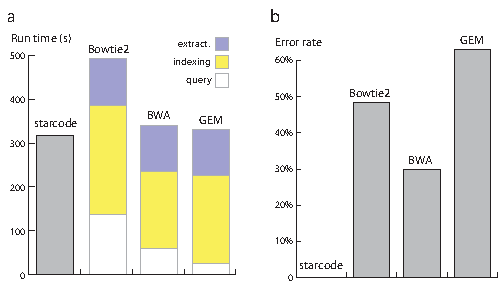
\includegraphics[scale=0.47]{benchmark.pdf}}
\caption{Accuracy of the sequence clustering and all-pairs search
algorithms. Starcode, seed and cd-hit were bencmarked on 4 datasets
with the same number of sequences, but different number of clusters
(see main text). \textbf{a} Starcode identifies the correct number
of clusters, while seed and cd-hit identify about 40 false positives
per true positive. \textbf{b} Slidesort identifies 5-10\% less
pairs than starcode. In both panels, the red line is first
bisector.}
\label{fig:benchmark}
\end{figure}

While starcode achieves perfect clustering on all 4 datasets, the
clustering achieved by seed and cd-hit is incomplete. Both tools
identify approximately 40 false clusters per true cluster on all
the datasets. We also observed that slidesort found 5-10\% less
3-matches than starcode on all the datasets. We were surprised by
this result because slidesort is claimed to be an exact algorithm.
However, this was clearly not the case when we ran additional tests
on smaller datasets where naive pairwise comparisons is feasible
(the starcode repository contains such a dataset along with the
instructions to reproduce our observations, see
http://github.com/gui11aume/starcode/misc).

The running time of the different tools as a function of the size
of the clusters is shown on Figure \ref{fig:benchmark}c. For seed
and cd-hit it decreases as the cluster size increases, whereas
for starcode and slidesort it increases. In spite of this trend,
the performance of starcode remains competitive, even for clusters
of 1 million sequences. The memory usage is shown in Figure
\ref{fig:benchmark}c.
In conclusion, starcode was the only tool to achieve perfect precision
on these datasets. It also maintains competitive performance in
running time and memory usage.


%% Biological datasets %%
The performance on artificial data is not always in agreement with
the performance on experimental datasets. In typical experiments,
the sizes of the clusters may be uneven, and the reads may contain
near constant regions that may degrade the performance.
We benchmarked sequence clustering algorithms on the problem of
clustering TRIP barcodes \citep{pmid23953119}. Briefly, the principle
of TRIP (Thousands of Reporters Integrated in Parallel) is to tag
reporter transcripts with random barcodes and measure the abundance
of barcodes in the RNA as a proxy for gene expression. There is no
reference to match aberrant barcodes against, because the tagging
sequences are unknown.

The basic properties of the datasets used for benchmarking are
summarized in Table~\ref{tab:biobench_properties}. Datasets 1 and 2
consist of Illumina single reads; they differ by the total read count
and by the empirical cluster sizes. According to the output of starcode,
the largest clusters of dataset 1 contain approximately 2,000 sequences,
while dataset 2 contains 4 clusters with more than 1 million sequences.
Dataset 3 consist of Illumina paired-end reads.

\begin{table}[h]
\centering
\caption{Summary of the biological datasets used for benchmarking.
All the datasets are Illumina reads.}
\begin{tabular}{l|l c r}
    \textit{dataset}   & \textit{read count} &
    \textit{read length} & \textit{type} \\ \hline
    dataset 1 & 16,457,527   & 50  & single      \\
    dataset 2 & 127,675,537  & 50  & single      \\
    dataset 3 & 2,460,226    & 100  & paired-end \\
\end{tabular}
\label{tab:biobench_properties}
\end{table}

The running times of starcode, seed, slidesort, rainbow and cd-hit-est
are summarized in Table~\ref{tab:biobench_runtime}. Starcode was faster
than the other tools on all the datasets. Seed came in second position
on datasets 1 and 2, with a running time approximately 800 and 20 times
greater, respectively. Rainbow came in second position on dataset 3,
but it is the only other tool able cluster paired-end reads. We did not
record the exact running times past 10 days since this is several
orders of magnitude higher than the running time of starcode.

\begin{table}[h]
\centering
\caption{Running time (in seconds) of the software on three biological
datasets. Runs longer than 10 days were interrupted. A dash indicates
that the software cannot be used for this dataset.}
\begin{tabular}{l|c c c}
    \textit{software}   & \textit{dataset 1} &
      \textit{dataset 2} & \textit{dataset 3} \\ \hline
    starcode   & 171         & 2,898       & 44    \\
    seed       & 135,959     & 60,374      & -     \\
    sidesort   & 632,168     & $>$ 10 days & -     \\
    rainbow    & -           & -           & 306   \\
    cd-hit-est & $>$ 10 days & 512,591     & -     \\
\end{tabular}
\label{tab:biobench_runtime}
\end{table}

The memory footprint of the different tools on the same datasets is
shown in Table~\ref{tab:biobench_memory}. The values represent the
peak memory usage throughout the run on the datasets described above.
On datasets 1 and 3, starcode had a significantly larger memory usage
than the best tool, while on dataset 2 it used significantly less
memory than seed and approximately as much as cd-hit. A large portion
of the memory usage of starcode is dedicated to the trie structures
used in the poucet search, which explains why starcode is in general
more memory-demanding than alternative tools.

\begin{table}[h]
\centering
\caption{Memory usage (in Gb).}
\begin{tabular}{l|c c c}
    \textit{software}   & \textit{dataset 1} &
      \textit{dataset 2} & \textit{dataset 3} \\ \hline
    starcode   & 9.4 & 30.9 & 5.2 \\
    seed       & 4.1 & 53.9 & -   \\
    sidesort   & 1.9 & 13.9 & -   \\
    rainbow    & -   & -  & 0.5   \\
    cd-hit-est & 3.8 & 28.5 & -   \\
\end{tabular}
\label{tab:biobench_memory}
\end{table}


%\subsection{Clustering TRIP barcodes}
%In the course of setting up the TRIP technology in our laboratory
%\citep{pmid23953119}, we realized the need to develop efficient
%algorithms to cluster similar sequences. Briefly, the principle of TRIP
%(Thousands of Reporters Integrated in Parallel) is to tag reporter
%transcripts with random barcodes and measure the abundance of barcodes
%in the RNA as a proxy for gene expression. There is no reference to
%match aberrant barcodes against, because the tagging sequences are
%unknown. Instead, barcodes are matched against each other and clustered
%by similarity to infer canonical sequences.
%
%We tested the efficiency of starcode on the TRIP dataset from
%\cite{pmid23953119}. In the experiment labeled mPGKA, we identified
%24.1 million (91\%) barcode-containing reads out of 26.6 million,
%consisting of approximately 223,000 and 220,000 unique barcode sequences
%for PCR replicates 1 and 2, respectively. Following the authors, we kept
%only the barcodes with at least 5 counts and performed clustering as
%described: ``First we sorted barcodes according to their counts. Then,
%for each barcode (starting from the most frequent one), we identified
%and removed all its mutant versions, defined as barcodes within a Hamming
%distance of 2.'' We implemented this method, here on referred to as the
%``sequential algorithm'' with the function call
%\texttt{stringDist(method='lv', maxDist=2)} from R the package
%\texttt{stringDist} \citep{R}.  When replacing the Hamming distance by
%the Levenshtein
%distance, starcode produced exactly the same output as the sequential
%algorithm. The running time of starcode averaged over the replicates was
%2.90 seconds, \textit{versus} more than 3 minutes 40 seconds, which
%represents a 75-fold speedup.
%
%The performance of the sequential algorithm relies on the arbitrary
%exclusion of reads with less than 5 counts, the main purpose of which
%is to reduce the computational burden. When all barcodes were kept,
%the average running time of starcode was 10.27 seconds, \textit{versus}
%$>$ 6 hours for the sequential algorithm. Using the Hamming distance,
%as the authors originally suggested, decreased the average running time
%of the sequential algorithm to about 3 hours and 30 minutes (and
%the output differed from that of starcode). Note that in all the cases
%mentioned above, starcode was run with a single core to compare the
%algorithms based on similar computer resources. In conclusion, the
%barcode clustering problem can be simplified by various tricks, but
%starcode brings down the running time to nearly instantaneous, and
%thereby obviates the need for such arbitrary heuristics.

\subsection{Identifying enriched sequence motifs}
\label{section:motifs}
Sequence motifs are thought to play an important role in DNA metabolism.
Key regulators, such as transcription factors, nucleosomes and non
coding RNAs have sequence preferences targeting them to the sites where
they act. Identifying those sequences is a way to pinpoint the
regulators and the mechanisms they are involved in. However, the
sequence motifs are not strictly identical at different sites, hence
they are better identified by inexact matching. This problem becomes
computationally difficult for long motifs (above 12-13 nucleotides)
because of the combinatorial scaling. But as motifs become longer, the
problem of identifying abundant inexact matches becomes similar to
barcode clustering. We reasoned that starcode could also be used for
the task of identifying biologically meaningful sequence motifs.

We set up a test based on the meningitis-causing agent
\textit{Neisseria meningitidis}. The genome of this bacterium is
interspersed with a frequent 12 bp sequence known as DNA uptake
sequence \citep{pmid10673000}. We extracted the 12-mers from both
orientations of �the 2.19 Mb genome, yielding 4.39 million 12-mers,
consisting of 2.77 million unique sequences. Clustering the 12-mers
with starcode within a Levenshtein distance of 2 took less than 45
seconds with 12 threads. We identified the known DNA uptake sequence
of \textit{Neisseria meningitidis} (ATGCCGTCTGAA) as the most abundant
12-mer, with 1466 exact and 2096 inexact hits. This result testifies
to the fact that starcode can be used to identify biologically
relevant motifs in bacterial genomes.

To test starcode on another application, we used the RNA-protein
interaction data produced by RNAcompete \citep{pmid19561594}. The
mammalian splicing factor SRSF1 is known to bind RNA GA-rich motifs,
but there is some disagreement about the motif that it recognizes
\citep{pmid23562324}. For each replicate of the human SRSF1 in the
RNAcompete dataset, we replaced the microarray signals by their rank
and extracted the 10-mers from the microarray probes. The 10-mers were
given a score equal to the rank of the probe they belong, and enriched
motifs were found using the sphere clustering of starcode with maximum
Levenshtein distance 2. The score of the most enriched 10-mer is thus
the sum of the ranks of all 10-mers within this distance. Clustering
the 6.3 million extracted 10-mers with 12 threads took about 20 seconds
for each replicate.  The most enriched 10-mers were AGGACACGGA,
AGGACACGGA, AGGACGGAGG, AGGACGGAGG, AGGACACGGA and AGGATACAGG. Except
for the last replicate, the motifs consist of AGGAC and GGA, with a
spacer of variable length. This suggests that the binding of SRSF1 to
RNA may involve a spacer sequence, which would explain the disagreement
between the motifs derived from 6-mers or 7-mers.

\section{Discussion and conclusion}
Through the parallel poucet search algorithm, starcode implements an
exact sequence clustering algorithm that can be faster than popular
heuristics. By design, starcode is tailored to process high throughput
sequencing data on multi-core platforms. Our benchmark shows that
starcode achieves perfect clustering on short random sequences in less
time than what is considered acceptable for heuristic searches. We also
show that starcode outperforms next generation read mappers in this
context. The software tools used for this benchmark are usually not
used for barcode or random sequence clustering. In this respect,
starcode fills a need arising from the development of barcoding
technologies.

The speed of starcode also makes it useful for other clustering
tasks, such as identifying enriched motifs in microbial genomes and
in experimental data. Here we have given two examples of such
applications. In the first, we recover a known enriched 12-mer in the
genome of \textit{Neisseria meningitidis}. In the second, we recover
the motif of the human RNA binding protein SRSF1 and notice that it
seems to consist of two halves separated by a linker. This hypothesis
is consistent with the fact that SRSF1 binds RNA through two
consecutive RNA Recognition Motifs (RRM) that are known to bind
3-4 nucleotides in a row\citep{pmid23253355}. The Levenshtein distance,
which incorporates insertions and deletions is more likely to capture
bi-partite binding motifs than position weight matrix representations.
The use of a clustering method to tackle this problem is unusual, but it 
it illustrates the potential advantages of distance-based approaches.

The current version of starcode has been primarily optimized for speed.
The memory footprint depends on the number of sequences to cluster
(because the sequences of the input set are loaded in memory as a set of
of tries) and on the mean number of matches per sequence. Every match is
stored in memory until the clustering phase, which may represent a large
overhead if the dataset is dense. As counterintuitive as it may seem,
long queries will usually impose a lower memory footprint because the
matches between the sequences are more sparse. We have shown that the
running time will also be shorter thanks to the lookup table
search (Figure \ref{fig:perf}c).

Perhaps the most surprising element of this study is that an exact
algorithm can compete with extremely fast heuristics. This will no
longer be true when clustering divergent sequences because the Levenshtein
distance will have to be increased, leading to exponentially longer
running times (Figure \ref{fig:perf}b). However, for the imporant
practical case that the divergence is driven by sequencing errors,
starcode illustrates that there is still room for algorithmic innovations
that can outperform heuristics. The idea of the poucet search seems
simple in retrospect, yet it is a powerful way to tap into the data
structuration provided by string sorting. This principle could find some
applications in algorithms used in various fields.


%%%%%%%%%%%%%%%%%%%%%%%%%%%%%%%%%%%%%%%%%%%%%%%%%%%%%%%%%%%%%%%%%%%%%%%%%%%%%%%%%%%%%
%
%     please remove the " % " symbol from \centerline{\includegraphics{fig01.eps}}
%     as it may ignore the figures.
%
%%%%%%%%%%%%%%%%%%%%%%%%%%%%%%%%%%%%%%%%%%%%%%%%%%%%%%%%%%%%%%%%%%%%%%%%%%%%%%%%%%%%%%


\section*{Acknowledgement}
We would like to thank Maria Chatzou for her precious feedback on the
preliminary version of this manuscript.

\paragraph{Funding\textcolon}
The research leading to these results has received funding from the
Government of Catalonia (Dept. of Economy and Knowledge) and the Spanish
Ministry of Economy and Competitiveness (Centro de Excelencia Severo Ochoa
2013-2017' (SEV-2012-0208). P.C. fellowship is partly financed by the
Spanish Ministry of Economy and Competitiveness (State Training Subprogram:
predoctoral fellowships for the training of PhD students (FPI) 2013).

\bibliographystyle{natbib}
%\bibliographystyle{achemnat}
%\bibliographystyle{plainnat}
%\bibliographystyle{abbrv}
%\bibliographystyle{bioinformatics}
%
%\bibliographystyle{plain}
%
\bibliography{document}


%\begin{thebibliography}{}
%\end{thebibliography}
\end{document}
